\documentclass[11pt, letterpaper]{article}
\usepackage[a4paper, top=2cm, bottom=2cm, left=1.5cm, right=1.5cm]{geometry}
\usepackage{float}        % <<< added for in place tables
\usepackage{graphicx}     % For including figures
\usepackage{amsmath}      % For math
\usepackage{booktabs}     % For nice tables
\usepackage{hyperref}     % For links
\usepackage{cite}         % For citations
\usepackage{pgfplots}     % <<< ADDED FOR PLOTTING
\pgfplotsset{compat=1.18} % <<< ADDED FOR PLOTTING

% Citation: Google Gemini heavily assisted with the formatting of figures/tables using pgfplots

\title{CS 431 Homework 03-04 SpMV on the CPU and GPU}
\author{David Haddad}
\date{\today}

\begin{document}

\maketitle

\section{Introduction}
This report analyzes the performance of Sparse Matrix-Vector Multiplication (SpMV) implemented on both a multi-core CPU using OpenMP (Homework03) and a GPU using CUDA (Homework04). The primary purpose of these assignments was to explore different storage methods for the matrices -- Coordinate (COO), Compressed Sparse Row (CSR), and ELLPACK (ELL) -- and then evaluate how they perform under parallel execution of a specific matrix computation (multiplying a sparse matrix with a dense vector). These tests were conducted on a single matrix in \texttt{cant.mtx} using the Talapas cluster (which I now know has 28, not 32, CPU compute nodes and, of course, uses NVIDIA GPUs). These results are only accurate for this particular matrix under this specific Matrix-Vector computation. Other matrix manipulations and computations commonly found in linear algebra would exhibit differing performance across storage formats, since we are only really testing how the computer accesses memory during a single multiplication.

\section{Implementation Strategy}
\subsection{CPU Parallelization (OpenMP)}
For the CPU implementation, I focused on parallelizing the \texttt{convert\_coo\_to\_csr} and \texttt{spmv\_coo} functions.
\begin{itemize}
    \item \textbf{Parallel Prefix Sum:} CSR conversion requires calculating row pointers, which in turn requires calculating a prefix sum. Homework02 gave the necessary insights to implement a prefix sum helper function to decrease this computational overhead.
    \item \textbf{Atomics vs. Locks:} After multiple tests with the COO SpMV kernel, the performance did not change. I experimented with using \texttt{omp\_set\_lock} and \texttt{\#pragma omp atomic}. Neither the atomics nor the locks showed linear speedup. I decided to use the lock code for a variety of analyses. The overhead of the locks is clearly still visible as compared to CSR, which does not have such requirements. 
\end{itemize}

\subsection{GPU Parallelization (CUDA)}
The GPU tested the CSR and ELL implementations using the CUDA platform. This portion of the assignment focuses more on memory coalescing (ELL explicitly and CSR through warps). Homework04 also involved the concepts of shared memory and how synchronization can be costly. In the naive implementation, shared memory is a huge bottleneck. Each thread must wait to access global memory before adding its value to the result vector. To minimize global memory writes, I used a parallel reduction to accumulate partial sums before writing the final dot product to the output vector. This tree-like reduction causes the threads to combine their results in a series of steps, only writing to global memory once per row.

\section{Performance Analysis}
\subsection{CPU Scaling: COO vs. CSR}
I tested the CPU implementation's scalability by varying the thread count from 1 to 28. I noted that when running on 32 threads, the expected speedup trend no longer held, as it did for 1-16 threads. This led me to discover that the compute nodes on Talapas have 28 cores per logical block/node. \textbf{Figure \ref{fig:scaling}} shows how the CSR format demonstrated near-perfect linear speedup. Unfortunately, the locks overhead in the COO format causes a plateau in speedup after we increase past four threads. The atomic version of the COO format was displaying confusing results and thus is not discussed in this report.

\begin{figure}[ht]
    \centering
    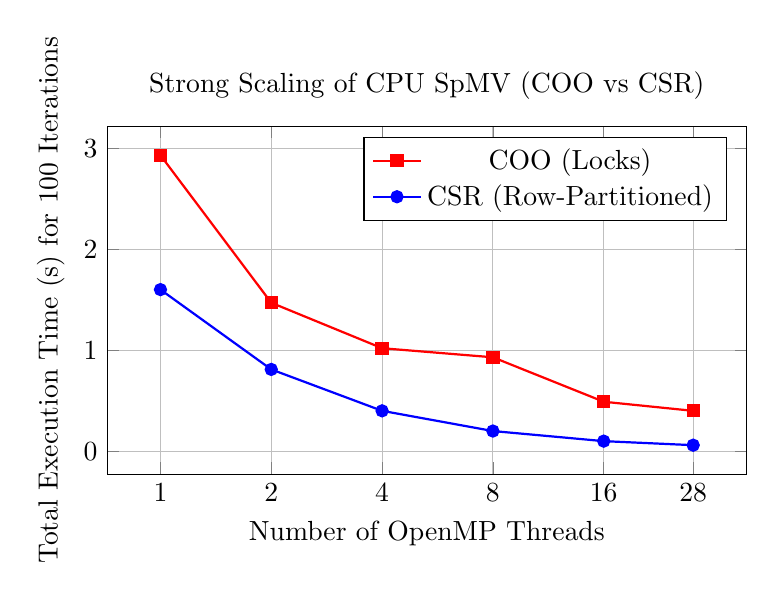
\begin{tikzpicture}
    \begin{axis}[
        width=0.8\textwidth,
        height=6cm,
        xlabel={Number of OpenMP Threads},
        ylabel={Total Execution Time (s) for 100 Iterations},
        xmode=log,
        log basis x={2},
        xtick={1,2,4,8,16,28},
        xticklabels={1, 2, 4, 8, 16, 28},
        grid=major,
        legend pos=north east,
        title={Strong Scaling of CPU SpMV (COO vs CSR)}
    ]
        % COO Data
        \addplot[color=red, mark=square*, thick] coordinates {
            (1, 2.93) (2, 1.47) (4, 1.02) (8, 0.93) (16, 0.49) (28, 0.40)
        };
        \addlegendentry{COO (Locks)}
        
        % CSR Data
        \addplot[color=blue, mark=*, thick] coordinates {
            (1, 1.60) (2, 0.81) (4, 0.40) (8, 0.20) (16, 0.10) (28, 0.06)
        };
        \addlegendentry{CSR (Row-Partitioned)}
    \end{axis}
    \end{tikzpicture}
    \caption{Execution time vs. thread count. CSR scales linearly, while COO struggles with lock overhead or atomic contention.}
    \label{fig:scaling}
\end{figure}


\subsection{CPU vs. GPU Comparison}
Comparing the best execution times for the CPU and the GPU highlights the latency differences between the two architectures. We expect to see a considerable speedup for the GPU, upwards of 10 times, but instead, the GPU is only roughly 1.5 times faster than the 28-core CPU CSR run. The most likely cause for this discrepancy is the matrix size. Modern GPUs are prepared to work with much larger datasets than our sample matrix \texttt{cant.mtx}. The time it takes to allocate and copy the input to the GPU is significantly longer than the time the GPU actually spends computing the result of our SpMV. This is why modern approaches consider more realistic situations in which the matrix is loaded into the GPU for hundreds or thousands of iterative computations (some SpMV, some not). This way, one can consider speedup and acceleration based on real-world computation scenarios rather than isolated test cases.

\begin{figure}[ht]
    \centering
    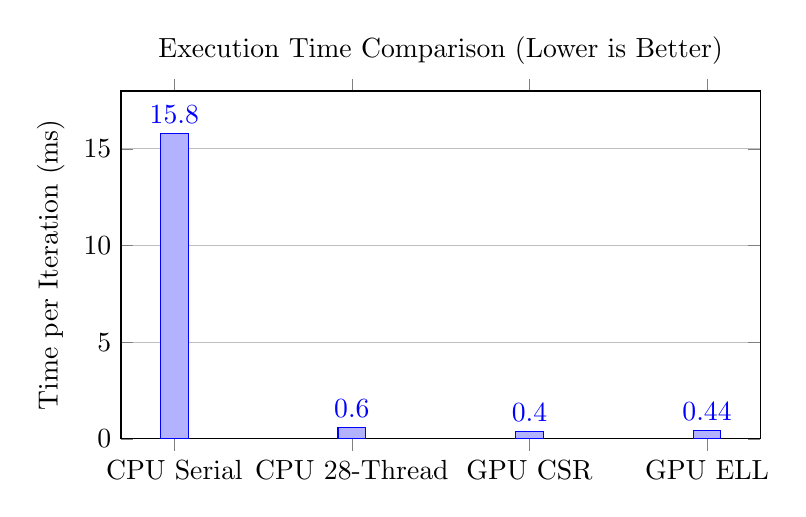
\begin{tikzpicture}
    \begin{axis}[
        ybar,
        width=0.8\textwidth,
        height=6cm,
        ylabel={Time per Iteration (ms)},
        symbolic x coords={CPU Serial, CPU 28-Thread, GPU CSR, GPU ELL},
        xtick=data,
        nodes near coords,
        ymin=0, ymax=18,
        ymajorgrids=true,
        title={Execution Time Comparison (Lower is Better)}
    ]
        \addplot coordinates {(CPU Serial, 15.8) (CPU 28-Thread, 0.6) (GPU CSR, 0.4) (GPU ELL, 0.44)};
    \end{axis}
    \end{tikzpicture}
    \caption{Per-iteration latency comparison. GPU CSR offers the lowest latency, marginally beating the highly parallel CPU CSR.}
    \label{fig:comparison}
\end{figure}

\section{Conclusion}
These two projects demonstrate the complex trade-offs programmers face when choosing storage format, algorithm structure, and computer architecture for large-scale code. Some formats, which may be easier to search, manipulate, and alter (COO), require atomic operations when computing Matrix-Vector products. CSR is superior for both the CPU and GPU because it uses memory more efficiently and allows rows to operate independently. This allows us as programmers to map the algorithm's structure neatly onto parallel constructs such as OpenMP pragmas and CUDA thread blocks/warps.



\end{document}